\documentclass[../ASSD_TP2.tex]{subfiles}
\begin{document}

\section{Algoritmo de Karplus Strong }

\subsection{Introducción}

El algoritmo de Karplus-Strong fue introducido en 1983 por Kevin Karplus
y Alex Strong, y consiste en la aplicación de ciertas técnicas digitales
para poder simular sonidos de instrumentos de manera sencilla y con
pocos recursos tanto físicos como digitales. En particular en este
trabajo práctico, se analizaran los modelos básico (también conocido
como punteo de guitarra), y una modificación para lograr reproducir
sonidos de instrumentos de percución.

\subsubsection{Modelo conceptual}

El modelo conceptual del algoritmo de Karplus-Strong consiste en excitar
un sistema linear con una secuencia aleatoria de longitud finita.
El sistema consiste en una línea de retardo de L muestras, realimentada
mediante un filtro como podemos observar en la figura \ref{fig:Diagrama-conceptual-del}. 

\begin{wrapfigure}{r}{0.5\columnwidth}%
\centering{}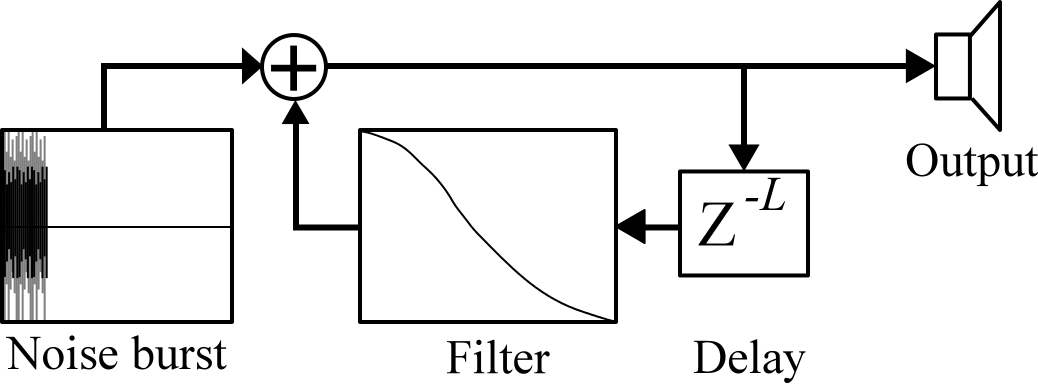
\includegraphics[scale=0.15]{imagenes/Karplus-strong-schematic}\caption{Diagrama conceptual del modelo básico de Karplus-Strong.\label{fig:Diagrama-conceptual-del}}
\end{wrapfigure}%

La idea principal es simular como los armónicos que recorre una cuerda
de longitud L, se van atenuando a medida que circulan por la misma.
Combinados con el filtro pasabajos, logramos que las frecuencias más
altas se atenúen aún más rápido y logramos mejorar la calidad del
audio que se percibe.

La primera aproximación al diagrama de la figura \ref{fig:Diagrama-conceptual-del}
es consiste en promediar dos muestras consecutivas, lo que produce
una atenuación progresiva de la señal entrante al sistema. Matemáticamente
se expresa de la siguiente manera: 
\begin{center}
$\begin{cases}
Y_{n}=\frac{1}{2}\cdot(Y_{n-p}+Y_{n-p-1}) & con\,p\epsilon\mathbb{N}\\
Y_{n}=\begin{cases}
+A & con\,probabilidad\,0.5\\
-A & con\,probabilidad\,0.5
\end{cases} & para\,-p\leq t\leq0
\end{cases}$
\par\end{center}

Este algoritmo logra emular perfectamente como el sonido de una cuerda
decae en el tiempo. Posee un período de $p+\frac{1}{2}$ muestras
($\frac{f_{s}}{p+1/2}$). Sin importar la forma que toma la señal
ni su contenido armónico, eventualmente siempre tiende a un valor
constante (manifestado en ``silencio''). No obstante, el sonido
resultante va a variar según las condiciones iniciales dadas. Para
lograr un mejor efecto, es conveniente que la señal tenga una gran
cantidad de armónicos de alta frecuencia. Para ello, $Y_{n}$ se genera
con valores aleatorios de valores $\pm A$, con igual probabilidad,
lo que hace que la señal tenga un gran contenido armónico pero además
esta libre de ruido.

\subsubsection{Variación para instrumentos de percusión}

Teniendo el modelo básico desarrollado anteriormente, es posible aplicarle
una variante para lograr sintetizar instrumentos de percución. Esta
variante consiste en mezclar los valores de las muestras medios con
su recíproco para así obtener el sonido. Matemáticamente, pued expresarse
de la siguiente manera:

$Y_{n}=\begin{cases}
+\frac{1}{2}\text{·}(Y_{n-p}+Y_{n-p-1}) & probabilidad\,b\\
-\frac{1}{2}\text{·}(Y_{n-p}+Y_{n-p-1}) & probabilidad\,1-b
\end{cases}$

El valor b, conocido como factor de mezcla, es el que determina la
proporción de comonentes realimentadas positiva y negativamente. Para
valores de $b\epsilon[0.1;0.6]$ se logran sonidos similares a intrumentos
de percusión. Notese que si b=1, obtenemos el algoritmo clásico del
sonido de guitarra.

\begin{figure}[H]

\begin{centering}
\includegraphics{\string"imagenes/diagrama modelo extendido\string".png}\caption{Diagrama conceptual del modelo extendido.}
\par\end{centering}
\end{figure}


\subsection{Análisis de ambos modelos}

Como a cualquier filtro digital, para el algoritmo Karplus-Strong
es posible encontrar su función transferencia (tanto para el filtro
convencional como a su modificación).

Para el modelo clásico, se puede obtener la función transferencia
Z mediante relaciones de recursión, obteniendose:
\begin{center}
$H(Z)=\frac{\frac{1}{2}\cdot(z^{-1}-1)\cdot z^{-p}}{1-\frac{1}{2}\cdot(z^{-1}-1)\text{·}z^{-p}}=\frac{1+z}{2z^{p+1}-z-1}$
\par\end{center}

Los polos se pueden encontrar igualando la expresión $2z^{p+1}-z-1=0$,
mientras que existe un único cero en $z=-1$, correspondiente a la
frecuencia de Nyquist $\frac{1}{2f_{s}}.$

\begin{wrapfigure}{r}{0.5\columnwidth}%
\centering{}\includegraphics[scale=0.5]{\string"imagenes/polos simple\string".png}\caption{Constelación de polos del modelo simple.}
\end{wrapfigure}%

Aproximando la fórmula de la expresión de los polos a $2\cdot z^{p+\frac{1}{2}}=z^{\frac{1}{2}}+z^{-\frac{1}{2}}$,
y asumiendo que los polos son de la forma $a\cdot e^{j\omega}$, la
expresión resultante es:
\begin{center}
$2\cdot a^{p+\frac{1}{2}}e^{j\omega(p+\frac{1}{2})}=a^{\frac{1}{2}}e^{j\omega/2}+a^{-\frac{1}{2}}e^{-j\omega/2}$
\par\end{center}

Aproximando $e^{j\omega(p+1/2)}\approx1$, podemos despejar $\omega=\frac{2\pi n}{(p+\frac{1}{2})}$.
Aproximando $2\cdot a^{p+1/2}\approx2cos(\frac{\omega}{2})$ podemos
despejar el tiempo de caída del n-esimo armónico siendo $a=(cos(\frac{2\pi n}{2p+1}))^{\frac{1}{p+\frac{1}{2}}}$. 

Para el modelo de percución, necesitamos otro tipo de análisis, puesto
que la señal que produce es aperiodica. Descomponiendo el sistema
en etapas, podemos expresar la función transferencia de la siguiente
manera:

\begin{wrapfigure}{l}{0.5\columnwidth}%
\centering{}\includegraphics[scale=0.5]{\string"imagenes/polos extendido\string".png}\caption{Constelación de polos del modelo extendido.}
\end{wrapfigure}%

\begin{center}
$H(z)=\frac{1}{1-H_{a}(z)*H_{b}(z)},con\,H_{a}(z)=\frac{1+z^{-1}}{2},H_{b}(z)=z^{-n}$
\par\end{center}

Sabiendo que $H(j\omega)=H(z=e^{j\omega}),$ podemos expresar las
funciones de ganancia y fase de la siguiente manera:
\begin{center}
$\begin{cases}
G_{a}(f)=|cos(\frac{\omega}{4\pi f_{s}})|\\
G_{b}(f)=1
\end{cases}$ ~~~ $\begin{cases}
P_{a}(f)=\frac{1}{2}\\
P_{b}(f)=N
\end{cases}$
\par\end{center}

Con estos parámetros, podemos calcular la ganancia de lazo $G=G_{a}\cdot G_{b}=cos(\pi fT_{s})$
y la longitud de lazo que es igual a $P_{a}+P_{b}=N+\frac{1}{2}$.

\subsection{Modelo conceptual básico}

\subsubsection{Estabilidad}

Conociendo la función transferencia del sistema, la condición para
que el mismo sea estable es que todos sus polos estén dentro del círculo
unitario, puesto que la función es causal.

Sabiendo que los polos son de la forma $a\cdot e^{j\omega}$, entonces
si $|z|<1\rightarrow|a\cdot e^{j\omega}|<1\rightarrow|a|<1$

Como $a=(cos(\frac{2\pi n}{2p+1}))^{\frac{1}{p+\frac{1}{2}}}$ entonces
$a\neq1$ lo que implica que $cos(c)\neq1$ lo que significa que $c\neq k\pi$,
por lo que la expresión final queda como:
\begin{center}
$\frac{2\pi n}{2p+1}\neq k\pi\Rightarrow n\neq k\cdot(p+\frac{1}{2})$
\par\end{center}

siendo n la longitud de la cuerda.

\subsubsection{Sintonización}

Uno de los problemas que el modelo básico accarrea en sí, es el hecho
de que la longitud de la cuerda L debe ser un número entero. Esto
ocaciona que las frecuencias fundamentales de la cuerda que se quiera
generar estén cuantizadas. Siendo $f=\frac{f_{s}}{N+0.5}$, a medida
que N es más chico, la diferencia entre N y N+0.5 es mucho más notoria,
lo que termina manifestandose en el dibujo y empeorando la calidad
del sonido.

\begin{figure}[H]

\begin{centering}
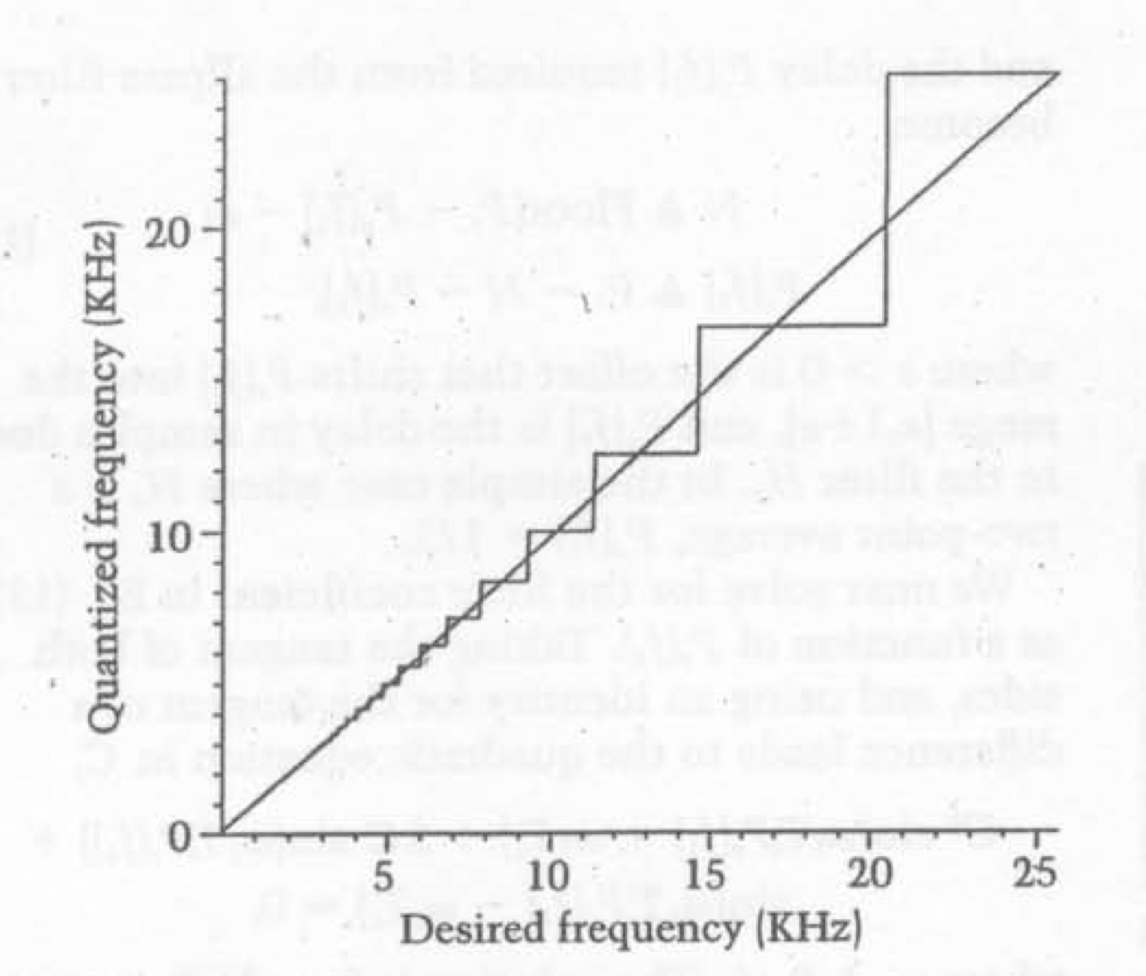
\includegraphics[scale=0.6]{imagenes/grafico1}\caption{Gráfico de la cuantización de la frecuencia.}
\par\end{centering}
\end{figure}

Una de las posibles soluciones a este inconveniente, es la de colocar
un filtro pasatodo en la realimentación del sistema para aplicar un
pequeño retardo de fase sin alterar la ganancia del mismo, el cual
esta dado por la siguiente ecuación:
\begin{center}
$H_{c}(z)=\frac{C+z^{-1}}{1+C\cdot z^{-1}}$
\par\end{center}

donde C es una constante que define el nuevo retardo del lazo, y se
calcula mediante la siguiente expresión:
\begin{center}
$C=\frac{sin(2\pi\cdot f_{1}T_{s})-sin(2\pi\text{·}f_{1}T_{s}\cdot P_{c}(z))}{sin(2\pi\text{·}f_{1}T_{s}+2\pi\text{·}f_{1}T_{s}\text{·}P_{c}(z))}=\frac{sin(2\pi\text{·}f_{1}T_{s}-2\pi\text{·}f_{1}T_{s}\text{·}P_{c}(z))}{sin(2\pi\text{·}f_{1}T_{s}+2\pi\text{·}f_{1}T_{s}\text{·}P_{c}(z))}$
\par\end{center}

donde $P_{c}(z)$ es la fase del filtro pasatodos, que se puede expresar
como $P_{c}(z)=N-floor(N-\varepsilon)$

\subsection{Modelo extendido }

\subsubsection{Fase en función de la probabilidad b}

Teniendo en cuenta que por el análisis hecho previamente conocemos
la función transferencia del sistema, podemos hallar la fase en función
de la probabilidad b. Sabiendo que $H(j\omega)=H(z=e^{j\omega}),$
y utilizando la igualdad de Euler para números complejos podemos llegar
a que la fase $\Phi(f)$ se puede expresar como:
\begin{center}
$\Phi(f)=tan(\frac{b\cdot sin(\frac{2\pi}{f_{s}}\cdot n+\pi\cdot\frac{1}{f_{s}})\cdot cos(\pi\text{·}\frac{1}{f_{s}})}{1-b\cdot cos(\frac{2\pi}{f_{s}}\text{·}n+\pi\text{·}\frac{1}{f_{s}})\text{·}cos(\pi\text{·}\frac{1}{f_{s}})}$
\par\end{center}

\subsubsection{Aplicaciones del paper ``Extensions of the Karplus Strong Algorithm''}

El paper realiza una serie de mejoras las cuales modifican el diseño
del algoritmo original para perfeccionarlo y lograr un sonido aún
más realista. Una de las series de mejoras que implementa es el filtro
dinámico, que controla la intensidad con la que se toca una cuerda.
Cuanto mayor es la intensidad en la misma, más energía poseen las
frecuencias más altas, efecto que no se ve reflejado en el algoritmo
original. Para lograrlo, se sugiere el siguiente filtro:
\begin{center}
$y(n)=(1-R)\cdot x(n)+R\cdot y(n-1)$
\par\end{center}

La función transferencia del filtro queda conformada:
\begin{center}
$H(z)=\frac{1-R}{1-R\cdot z^{-1}}$
\par\end{center}

Donde R es función de la frecuencia deseada y la longitud del arreglo
de muestras, y puede ser aproximado a $R=e^{-\pi L}$.

Otra de las mejoras que ofrece el paper, es la posibilidad de alargar
o acortar los tiempos de decaimiento del sonido. Para acortar el tiempo
de decaimiento, basta con multiplicar al algoritmo por una constante
$\rho<1$, tal que $\rho=0.99\cdot\frac{1-(1000\cdot duraci\acute{o}n)^{-1}}{1+(1000\text{·}duraci\acute{o}n)^{-1}}$.
Ahora, el sistema pasa a ser:
\begin{center}
$Y_{n}=\rho\cdot\frac{1}{2}\text{·}(Y_{n-p}+Y_{n-p-1})$
\par\end{center}

Si lo que se desea es alargar el tiempo de decaimiento, lo que debemos
modificar es el lazo de realimentación dado por $H_{a}(z)$, de manera
tal de que ahora sea $H_{a}(z)=(1-s)+s\cdot z^{-1}$, donde $0<s<1$
es el factor de estiramiento. Con esto en cuenta, ahora la ganancia
de lazo queda conformada:
\begin{center}
$G_{a}(z)=\sqrt{(1-s)^{2}+s^{2}+2s(1-s)\cdot cos(2\pi f\cdot T_{s})}$
\par\end{center}

\subsection{Conclusiones}

El Algoritmo de Karplus Strong es un algoritmo fácil y rápido que
nos permite emular el sonido de una cuerda de guitarra con mucha precisión.
Es un modelo versatil, puesto que con menores modificaciones no solo
se pueden lograr sonidos de otros instrumentos como los de percusión,
sino que también es posible de mejorar la calidad del sonido que se
sintetiza.

\end{document}
